\documentclass[a4paper,12pt]{article}
\usepackage[utf8]{inputenc}
\usepackage[spanish]{babel}
\usepackage{graphicx}
\graphicspath{{./figuras/}}
\usepackage[a4paper, left=2cm, right=2cm, top=2.5cm, bottom=2.5cm]{geometry}
\usepackage{xcolor} % Añadido para usar colores
\usepackage{amsmath}
\usepackage{float}

% Definir un color para los títulos (puedes ajustar el color como quieras)
\definecolor{azulUPP}{RGB}{0,70,128} % Un azul corporativo o tecnológico

% Redefinir el formato de las secciones y subsecciones para incluir color
\usepackage{titlesec}
\titleformat{\section}{\Large\bfseries\color{azulUPP}}{}{0em}{\MakeUppercase}[]
\titleformat{\subsection}{\large\bfseries\color{azulUPP}}{}{0em}{}[]
\titleformat{\subsubsection}{\bfseries\color{azulUPP}}{}{0em}{}[]

\begin{document}
	% Portada
	\begin{titlepage}
		\centering
		% Logos institucionales y nombre de la universidad
		
\includegraphics[width=0.25\textwidth]{logoUpp} \hspace{7cm} 
		
\includegraphics[width=0.25\textwidth]{logoSftw}
		\vspace{2cm}
		
		\Huge \textbf{Universidad Politécnica de Pachuca}\\
		\vspace{0.5cm}
		\Large Ingeniería en Software
		\vspace{1cm}
		
		% Titulo
		\Huge \textbf{Conceptos Teóricos - Proyecto de Tercer Parcial.}
		\vspace{1cm}
		
		% Información completa
		\Large \textbf{Materia:} Arquitectura de computadoras \\
		\Large \textbf{Docente:} Víctor Hainy\\
		\vspace{1cm}
		\Large \textbf{Alumno:} \\Peña Serrano José Abraham\\
		\vspace{1cm}
		\Large \textbf{Matricula:} \\2331123273\\
		\vspace{1cm}
		\Large \textbf{Grupo:} SFTW\_06\_01\\
		\vspace{1cm}
		\Large \textbf{Cuatrimestre:} Mayo - Agosto 2025
		
	\end{titlepage}
	
	\tableofcontents
	
	\newpage
	\section{Objetivo de aprendizaje}
	Describir el uso y funcionamiento de los microcontroladores, actuadores y sistemas embebido en sistemas reales aplicados.
	
	\section{Conceptos Teóricos}
	
	\subsection{Microcontroladores}
	\subsubsection{Definición}
	Un \textbf{microcontrolador} es un circuito integrado que incluye en un solo chip los elementos esenciales de un sistema informático: una unidad central de procesamiento (CPU), memoria (RAM y ROM/Flash) y periféricos de entrada/salida (E/S). A diferencia de los microprocesadores convencionales, los microcontroladores están diseñados para controlar dispositivos específicos o sistemas embebidos, realizando tareas concretas de manera automática y eficiente. Se encuentran en aplicaciones tan variadas como electrodomésticos, automóviles, sistemas de automatización industrial y dispositivos médicos.
	
	El microcontrolador es el “cerebro” de sistemas electrónicos autónomos, permitiendo la interacción con el entorno y la automatización de tareas específicas sin requerir la intervención continua de un usuario.
	
	\subsubsection{Tipos}
	Existen varios criterios para clasificar los microcontroladores, siendo los más comunes:
	
	\begin{itemize}
		\item \textbf{Por arquitectura:}
		\begin{itemize}
			\item \textit{Basados en arquitectura Harvard:} Separan físicamente la memoria de instrucciones y de datos (por ejemplo, la familia PIC).
			\item \textit{Basados en arquitectura Von Neumann:} Comparten el mismo bus para instrucciones y datos (como algunos modelos de 8051).
		\end{itemize}
		\item \textbf{Por tamaño de palabra (bits):}
		\begin{itemize}
			\item Microcontroladores de 8 bits: Los más extendidos en aplicaciones sencillas y de bajo costo, como el 8051 o los PIC de gama baja.
			\item Microcontroladores de 16 bits: Ofrecen mayor capacidad de procesamiento para sistemas más complejos.
			\item Microcontroladores de 32 bits: Destinados a aplicaciones que requieren alto rendimiento, como ARM Cortex-M usados en IoT y entornos industriales.
		\end{itemize}
		\item \textbf{Por fabricante/familia:}
		\begin{itemize}
			\item 8051: Amplia trayectoria en aplicaciones industriales y educativas.
			\item PIC: Desarrollados por Microchip, populares en electrónica y automatización.
			\item AVR: Utilizados en plataformas Arduino, ideales para prototipado educativo.
			\item ARM: Reconocidos por eficiencia y potencia, usados en aplicaciones comerciales.
		\end{itemize}
	\end{itemize}
	
	\subsubsection{Componentes y Características}
	Los microcontroladores integran los siguientes \textbf{componentes principales}:
	
	\begin{itemize}
		\item \textbf{CPU (Unidad Central de Procesamiento):} La parte que ejecuta instrucciones y procesa datos.
		\item \textbf{Memoria RAM:} Almacenamiento temporal para datos en ejecución.
		\item \textbf{Memoria ROM/Flash:} Almacena el programa y datos permanentes; puede ser reprogramable.
		\item \textbf{Periféricos de Entrada/Salida (E/S):} Puertos digitales, ADC, PWM, interfaces de comunicación (USART, SPI, I2C, CAN, USB, etc.).
		\item \textbf{Temporizadores y contadores:} Para controlar eventos temporales.
		\item \textbf{Convertidores Analógico-Digital (ADC) y Digital-Analógico (DAC):} Para manejo de señales analógicas.
		\item \textbf{Módulos de comunicación:} UART, SPI, I2C, CAN, que permiten interacción con otros dispositivos.
		\item \textbf{Reloj interno o externo:} Para sincronización y control del rendimiento.
	\end{itemize}
	
	Entre sus \textbf{características} destacan:
	
	\begin{itemize}
		\item Bajo consumo energético y modos de ahorro de energía.
		\item Tamaño compacto y bajo costo.
		\item Facilidad de reprogramación y vasto soporte en herramientas de desarrollo.
		\item Resistencia a ambientes adversos con encapsulados específicos.
	\end{itemize}
	
	\subsubsection{Proceso de Selección}
	
	El microcontrolador ESP32-WROOM-32 cumple con los criterios de selección para HYDROWARE, los cuales son:
	
	\begin{itemize}
		\item \textbf{Tipo de aplicación:} El ESP32 es ideal para sistemas IoT (Internet de las Cosas) de monitoreo. Su capacidad para manejar múltiples sensores y la comunicación inalámbrica se adapta perfectamente a la complejidad del sistema HYDROWARE.
		\item \textbf{Cantidad y tipo de entradas/salidas necesarias:} Cuenta con suficientes pines GPIO (General-Purpose Input/Output) para conectar el sensor de temperatura DS18B20, el sensor de pH y el display LCD 2x16. Además, maneja entradas y salidas digitales y analógicas necesarias.
		\item \textbf{Memoria requerida:} El ESP32 dispone de memoria SRAM y Flash que son suficientes para el código del sistema, el registro de datos y la gestión de la aplicación móvil.
		\item \textbf{Velocidad y capacidad de procesamiento:} Su procesador de doble núcleo (Dual-Core) ofrece la capacidad de procesamiento necesaria para leer datos de los sensores, procesar la información y gestionar la conectividad inalámbrica de manera simultánea y eficiente.
		\item \textbf{Interfaces de comunicación:} La integración de Wi-Fi y Bluetooth es crucial para el proyecto. El Wi-Fi permite la comunicación con la aplicación móvil y la visualización de datos en tiempo real, mientras que el Bluetooth podría ser usado para la configuración inicial o comunicación a corta distancia.
		\item \textbf{Consumo de energía:} El ESP32 ofrece modos de bajo consumo (Deep Sleep) que son beneficiosos para optimizar la duración de la batería.
		\item \textbf{Disponibilidad de soporte técnico:} El ESP32 tiene una vasta comunidad de desarrolladores, documentación detallada, librerías y herramientas de programación (IDE de Arduino, PlatformIO), lo que facilita su desarrollo y depuración.
		\item \textbf{Costo y disponibilidad:} Es un microcontrolador de bajo costo y fácil de conseguir en el mercado, lo que lo hace accesible para proyectos como HYDROWARE.
	\end{itemize}
	
	El ESP32-WROOM-32 se alinea con todos los factores clave del proceso de selección, garantizando la eficiencia, funcionalidad y viabilidad del sistema de monitoreo automatizado HYDROWARE.
	\vspace{0.5cm}
	%\noindent \textit{Referencias:} \\
	%Raúl A. Aquino Santos y Marien N. Rivera Gutiérrez, \textit{Microcontroladores. Fundamentos y aplicaciones}. \\
	%Microchip Technology, \textit{What is a Microcontroller?} \\
	%Texas Instruments, \textit{Selecting a Microcontroller}. 
	

	
	\subsection{Instrucciones de microcontroladores}
	Las instrucciones de microcontroladores son el lenguaje de máquina que el procesador entiende directamente. Aunque el lenguaje de programación de alto nivel como C++ se utiliza para el desarrollo, este es compilado a un lenguaje de ensamblador y luego a código de máquina para ser ejecutado por el microcontrolador.
	
	\subsubsection{Sintaxis de Instrucciones}
	La sintaxis de las instrucciones en el lenguaje de ensamblador, que es el puente entre el código de alto nivel y el código de máquina, sigue una estructura bien definida. Esta sintaxis permite al programador escribir código de una manera legible antes de que sea convertido a su forma binaria. La estructura general es la siguiente:
	
	\begin{verbatim}
		[etiqueta] opcode [operando1], [operando2], ... ; [comentario]
	\end{verbatim}
	
	Cada componente tiene un rol específico:
	\begin{itemize}
		\item \textbf{Etiqueta (\textit{label}):} Es un identificador simbólico opcional que se coloca al inicio de una línea. Funciona como un marcador de posición para una dirección de memoria en particular. Las etiquetas son vitales para la legibilidad y la programación estructurada, ya que permiten hacer saltos (\texttt{JMP}) o llamadas a subrutinas (\texttt{CALL}) sin necesidad de conocer la dirección de memoria exacta.
		\item \textbf{Opcode (\textit{Operation Code}):} Es el elemento principal de la instrucción. Es un mnemónico que representa una operación específica que el microcontrolador debe realizar. Por ejemplo, en la arquitectura del ESP32, un \texttt{MOV} podría mover un dato, un \texttt{ADD} podría sumar dos valores, y un \texttt{JMP} podría cambiar el flujo de ejecución del programa.
		\item \textbf{Operandos (\textit{operands}):} Son los datos o las ubicaciones de memoria que la instrucción va a manipular. El número de operandos depende del tipo de instrucción. Pueden ser:
		\begin{itemize}
			\item \textit{Registros:} Almacenes de datos de alta velocidad dentro de la CPU (por ejemplo, \texttt{R1}, \texttt{R2}).
			\item \textit{Valores inmediatos:} Datos constantes que se incluyen directamente en la instrucción (por ejemplo, el número `10`).
			\item \textit{Direcciones de memoria:} Ubicaciones en la RAM o en la memoria Flash donde se encuentran los datos.
		\end{itemize}
		\item \textbf{Comentario (\textit{comment}):} Todo lo que sigue a un delimitador (como un punto y coma \texttt{;}) en una línea es un comentario. El ensamblador lo ignora, pero es fundamental para que el código sea comprensible para los humanos, documentando la lógica y el propósito de cada instrucción.
	\end{itemize}
	
	\vspace{0.5cm}
	
	\textbf{Ejemplo de una instrucción simple:}
	\begin{verbatim}
		INICIO: MOV A, #50 ; Carga el valor 50 en el registro A
	\end{verbatim}
	En este ejemplo:
	\begin{itemize}
		\item \texttt{INICIO} es la etiqueta.
		\item \texttt{MOV} es el opcode (mover).
		\item \texttt{A} y \texttt{\#50} son los operandos (mover el valor 50 al registro A).
		\item `Carga el valor 50 en el registro A` es el comentario.
	\end{itemize}
	\subsubsection{Estructura de las Instrucciones}
	A nivel de máquina, cada instrucción de un microcontrolador se representa como una serie de bits con una estructura específica que la CPU puede decodificar y ejecutar. Esta estructura, que es la forma binaria de las instrucciones de ensamblador, típicamente se compone de los siguientes campos:
	
	\begin{itemize}
		\item \textbf{Opcode (Código de Operación):} Es el campo fundamental de la instrucción. Ocupa los primeros bits y define de manera única la operación a realizar (por ejemplo, suma, resta, transferencia de datos). En una arquitectura de 32 bits como la del ESP32, el tamaño de este campo puede variar dependiendo de la complejidad de la instrucción.
		\item \textbf{Modo de Direccionamiento:} Este campo especifica cómo la CPU debe acceder a los operandos. Algunos modos comunes son:
		\begin{itemize}
			\item \textit{Inmediato:} El valor del operando está directamente en la instrucción.
			\item \textit{Directo:} La instrucción contiene la dirección de memoria donde se encuentra el operando.
			\item \textit{Registro:} El operando se encuentra en uno de los registros de la CPU.
		\end{itemize}
		\item \textbf{Campos de Registros o Direcciones:} Contienen los identificadores de los registros que se utilizarán en la operación o la dirección de memoria a la que se va a acceder. En instrucciones con múltiples operandos, como una suma (\texttt{ADD}), se especifican los registros de origen y destino.
	\end{itemize}
	
	Esta organización compacta y precisa permite que la CPU procese las instrucciones a una velocidad muy alta, realizando la acción deseada con los datos especificados.
	
	\subsubsection{Características y Tipos de Instrucciones}
	Las instrucciones de un microcontrolador se pueden clasificar en varias categorías funcionales que cubren todas las operaciones que el dispositivo puede realizar. En la familia de microcontroladores Xtensa, como el ESP32, se encuentran los siguientes tipos principales:
	
	\begin{itemize}
		\item \textbf{Instrucciones de transferencia de datos:} Estas instrucciones mueven datos entre diferentes ubicaciones, como entre registros, memoria RAM y memoria Flash. No alteran los datos, solo su ubicación.
		\begin{itemize}
			\item \texttt{MOV}: Mueve un dato de un lugar a otro.
			\item \texttt{LOAD}: Carga un dato desde la memoria a un registro.
			\item \texttt{STORE}: Almacena un dato de un registro en la memoria.
		\end{itemize}
		\item \textbf{Instrucciones aritméticas y lógicas:} Realizan operaciones matemáticas (suma, resta) y lógicas (AND, OR, XOR) con los datos. Son esenciales para el procesamiento de información y la toma de decisiones.
		\begin{itemize}
			\item \texttt{ADD}: Suma dos operandos.
			\item \texttt{SUB}: Resta dos operandos.
			\item \texttt{AND}, \texttt{OR}: Realizan operaciones lógicas a nivel de bits.
		\end{itemize}
		\item \textbf{Instrucciones de control de flujo:} Son cruciales para modificar el orden de ejecución del programa. Permiten la creación de bucles, condicionales y subrutinas.
		\begin{itemize}
			\item \texttt{JMP}: Salto incondicional a una dirección de memoria específica.
			\item \texttt{CALL}: Llama a una subrutina y guarda la dirección de retorno.
			\item \texttt{RET}: Retorna de una subrutina al punto de llamada.
		\end{itemize}
		\item \textbf{Instrucciones de manipulación de bits:} Permiten el control granular de bits individuales, lo cual es fundamental para interactuar con los pines de E/S y configurar periféricos.
		\begin{itemize}
			\item \texttt{SETB}: Establece un bit en 1.
			\item \texttt{CLRB}: Borra un bit, poniéndolo en 0.
		\end{itemize}
	\end{itemize}
	
	\subsubsection{Proceso de Codificación}
	El proceso de codificación de instrucciones es la serie de pasos que transforma el código fuente legible por humanos en el código binario ejecutable por el microcontrolador. Este flujo de trabajo se automatiza en gran medida por herramientas de desarrollo, como el IDE de Arduino. Los pasos principales son:
	
	\begin{enumerate}
		\item \textbf{Código Fuente:} El programador escribe el código en un lenguaje de alto nivel, como C++ para el ESP32. El código está lleno de lógica, funciones y librerías que simplifican el desarrollo.
		\item \textbf{Compilación:} El \textbf{compilador} (por ejemplo, `g++` para el ESP32) lee el código fuente en C++ y lo traduce a un archivo de lenguaje de ensamblador, que es un lenguaje de bajo nivel con instrucciones como \texttt{MOV} y \texttt{ADD}.
		\item \textbf{Ensamblaje:} El \textbf{ensamblador} toma el archivo de ensamblador y lo convierte en código objeto binario, que es un archivo que contiene las instrucciones en su forma binaria.
		\item \textbf{Vinculación (Linker):} El \textbf{enlazador} combina todos los archivos de código objeto, junto con las librerías necesarias (por ejemplo, las librerías para Wi-Fi o para el sensor de temperatura), en un único archivo ejecutable. Este archivo final es el \textit{firmware} que se cargará en el microcontrolador.
		\item \textbf{Carga (Flasheo):} Finalmente, el cargador de arranque del microcontrolador (bootloader) se encarga de transferir y escribir el archivo ejecutable en la memoria Flash del ESP32, donde residirá de manera permanente y se ejecutará al encender el dispositivo.
	\end{enumerate}
	
	
	\subsection{Programación de microcontroladores}
	La programación de microcontroladores consiste en el arte y la técnica de escribir código que interactúe con el hardware físico para controlar el comportamiento del dispositivo. Para lograr esto, es fundamental comprender cómo el microcontrolador gestiona y procesa las señales del mundo real a través de sus interfaces.
	
	\subsubsection{Interfaces de Microcontroladores}
	Una \textbf{interfaz de microcontroladores} es el conjunto de componentes de hardware y software que facilitan la comunicación y la transferencia de datos entre el microcontrolador y los periféricos externos. Sus características y tipos principales son:
	
	\begin{itemize}
		\item \textbf{GPIO (General-Purpose Input/Output):} Son los pines más versátiles del microcontrolador. Pueden ser configurados por software como entradas o salidas digitales, permitiendo la lectura de botones o el encendido de LEDs.
		\item \textbf{ADC (Convertidor Analógico-Digital):} Es una interfaz especializada que convierte señales analógicas (como las del sensor de pH) en valores digitales que el microcontrolador puede procesar. La resolución del ADC (en bits) determina la precisión de la conversión.
		\item \textbf{PWM (Modulación por Ancho de Pulso):} Genera señales digitales que simulan un comportamiento analógico, útil para controlar la intensidad de un LED o la velocidad de un motor.
		\item \textbf{Interfaces de Comunicación Serial:} Son protocolos de comunicación que permiten a los dispositivos intercambiar datos bit a bit. En el proyecto HYDRAWARE, se utilizan:
		\begin{itemize}
			\item \textit{One-Wire:} Protocolo bidireccional que utiliza un solo pin de datos para la comunicación. El sensor de temperatura DS18B20 emplea este protocolo.
			\item \textit{I2C (Inter-Integrated Circuit):} Protocolo serial de dos hilos (datos y reloj) que permite a múltiples dispositivos comunicarse con el microcontrolador. El display LCD 2x16 se conecta a través de I2C, lo que minimiza la cantidad de pines utilizados.
		\end{itemize}
	\end{itemize}
	
	\subsubsection{Interfaces y Señales}
	Para interactuar con el entorno físico, un microcontrolador debe ser capaz de manejar dos tipos de señales:
	
	\begin{itemize}
		\item \textbf{Señal Analógica:} Una señal continua en el tiempo que puede tomar cualquier valor dentro de un rango determinado. Por ejemplo, la temperatura ambiente o la medición del pH son variables físicas que se representan con señales analógicas.
		\item \textbf{Señal Digital:} Una señal discreta que solo puede tener un número limitado de estados, típicamente dos: \textit{Alto} (representado por 1) y \textit{Bajo} (representado por 0). Un interruptor encendido o apagado es un ejemplo de señal digital.
	\end{itemize}
	
	Los \textbf{sistemas digitales} se caracterizan por su precisión y resistencia al ruido, ya que operan con estados definidos (1 y 0). En contraste, los \textbf{sistemas analógicos} se utilizan para capturar la variabilidad del mundo real, pero pueden ser más susceptibles a la distorsión. La mayoría de los microcontroladores modernos, como el ESP32, están diseñados para operar de manera digital, por lo que utilizan convertidores para interpretar datos analógicos.
	
	
	
	\subsubsection{Periféricos de Entrada y Salida}
	Los periféricos son los dispositivos externos que interactúan con el microcontrolador. Se dividen en dos categorías:
	
	\begin{itemize}
		\item \textbf{Periféricos de Entrada:} Dispositivos que proporcionan datos al microcontrolador para su procesamiento.
		\begin{itemize}
			\item \textbf{Sensor de Temperatura Digital DS18B20:} Este sensor de entrada digital utiliza el protocolo \textit{One-Wire} para enviar lecturas de temperatura precisas. Es crucial para monitorear la salud de los peces en el proyecto HYDRAWARE.
			\item \textbf{Sensor de pH PH-4502C:} Es un sensor de entrada analógico. Mide el nivel de acidez o alcalinidad del agua y envía una señal analógica al ESP32 para que sea convertida a un valor digital a través del ADC.
		\end{itemize}
		\item \textbf{Periféricos de Salida:} Dispositivos que reciben señales del microcontrolador para ejecutar una acción o mostrar información.
		\begin{itemize}
			\item \textbf{Display LCD 2x16:} Este es un periférico de salida digital que recibe datos del microcontrolador a través de una interfaz I2C. Su función en HYDRAWARE es mostrar de manera local y en tiempo real las mediciones de temperatura y pH.
		\end{itemize}
	\end{itemize}
	
	\subsubsection{Proceso de Conexión y Programación}
	El proceso de implementación se divide en dos fases principales: la conexión física (hardware) y el desarrollo lógico (software).
	
	\paragraph{Proceso de Conexión:}
	La conexión de los periféricos al ESP32 debe seguir una cuidadosa planificación:
	\begin{enumerate}
		\item \textbf{Identificación de Pines:} Se deben consultar las hojas de datos de todos los componentes para identificar los pines de alimentación (\textit{VCC}), tierra (\textit{GND}) y de datos.
		\item \textbf{Conexión del Sensor DS18B20:} El pin de datos del sensor se conecta a un pin GPIO del ESP32. Se requiere una resistencia \textit{pull-up} (generalmente de $4.7\text{k}\Omega$) entre el pin de datos y la alimentación para asegurar una comunicación estable del bus \textit{One-Wire}.
		\item \textbf{Conexión del Sensor de pH:} El módulo del sensor de pH se conecta a una fuente de alimentación de 5V y su pin de salida analógica se conecta a uno de los pines ADC del ESP32 para realizar la lectura.
		\item \textbf{Conexión del Display LCD:} El display LCD I2C se conecta a los pines de comunicación I2C del ESP32, que suelen ser GPIO 21 (SDA) y GPIO 22 (SCL).
	\end{enumerate}
	
	\paragraph{Proceso de Programación:}
	Una vez que el hardware está conectado, el microcontrolador necesita ser programado para realizar su función.
	\begin{enumerate}
		\item \textbf{Desarrollo del Firmware:} El código (firmware) se escribe en un entorno como el IDE de Arduino o PlatformIO, utilizando C++. Se incluyen librerías específicas para cada periférico (por ejemplo, `OneWire.h` y `DallasTemperature.h` para el sensor DS18B20, o librerías para la comunicación I2C del LCD).
		\item \textbf{Lógica del Programa:} El código debe incluir la lógica para inicializar las interfaces, leer los datos de los sensores, procesar los valores (por ejemplo, calibrar la lectura del pH), mostrar la información en el LCD, y establecer la comunicación inalámbrica (Wi-Fi) para enviar los datos a la aplicación móvil.
		\item \textbf{Carga al Microcontrolador:} El código compilado se transfiere a la memoria Flash del ESP32 a través de una conexión USB. Al reiniciar el dispositivo, el programa se ejecuta automáticamente, iniciando el proceso de monitoreo.
	\end{enumerate}
	
	
	\subsection{Sistemas embebidos}
	\subsubsection{Definiciones}
	\begin{itemize}
		\item \textbf{Sistema embebido:} Es un sistema informático especializado, diseñado para realizar una o varias funciones específicas dentro de un sistema más grande. A diferencia de una computadora de uso general, un sistema embebido se centra en la eficiencia, el bajo costo y el bajo consumo de energía. El sistema HYDRAWARE, al estar dedicado al monitoreo de agua, es un claro ejemplo de un sistema embebido.
		\item \textbf{Sensor:} Es un dispositivo que detecta y responde a un tipo de energía o señal física (como calor, luz, sonido, presión) y la convierte en una señal eléctrica o digital que el microcontrolador puede interpretar.
		\item \textbf{Actuador:} Es un dispositivo que convierte una señal de control (eléctrica o digital) del microcontrolador en un movimiento físico o una acción, como abrir una válvula, encender un motor o una bomba.
	\end{itemize}

	\subsubsection{Características y Tipos}
	Los sistemas embebidos se caracterizan por ser de propósito fijo, funcionar en tiempo real, ser de bajo consumo y compactos.
	\begin{figure}[h]
		\centering
		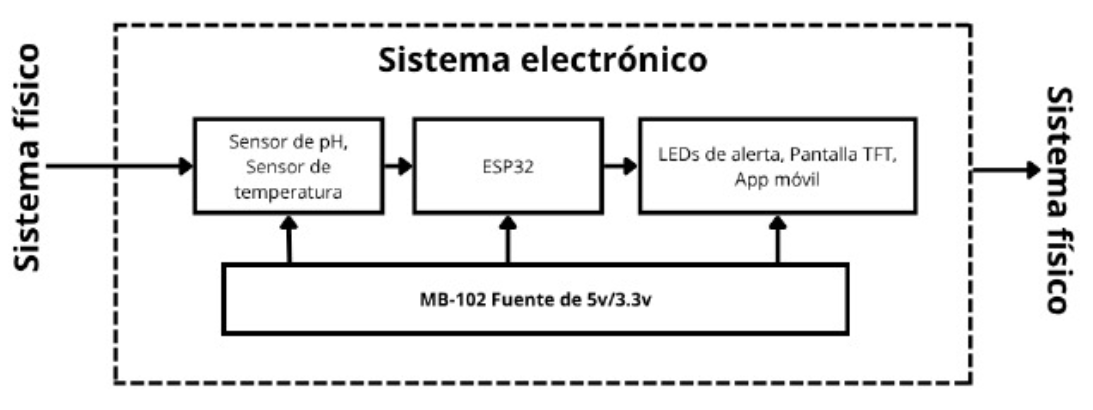
\includegraphics[width=0.9\textwidth]{diagrama.png}
		\caption{Diagrama de bloques de un sistema embebido}
	\end{figure}
	\begin{itemize}
		\item \textbf{Sistemas Embebidos:}
		\begin{itemize}
			\item \textit{En tiempo real:} Responden a eventos en un plazo de tiempo predecible. HYDRAWARE requiere esto para las alertas inmediatas.
			\item \textit{Autónomos:} Funcionan sin intervención humana continua.
			\item \textit{Tipos:} De red (como HYDRAWARE), móviles, o en tiempo real.
		\end{itemize}
		\item \textbf{Sensores y Actuadores:}
		\begin{itemize}
			\item \textit{Sensores:} \textbf{Analógicos} (PH-4502C) y \textbf{digitales} (DS18B20).
			\item \textit{Actuadores:} Aunque HYDRAWARE inicialmente es solo un sistema de monitoreo, podría expandirse con actuadores como una bomba para regular el pH.
		\end{itemize}
	\end{itemize}
		
	\subsubsection{Plataformas de Sistemas Embebidos}
	Una \textbf{plataforma de sistemas embebidos} es un ecosistema completo que proporciona el hardware, el software y las herramientas necesarias para diseñar y programar un sistema embebido. Estas plataformas simplifican el proceso de desarrollo al ofrecer un microcontrolador o microprocesador preensamblado en una placa de circuito, junto con un entorno de desarrollo integrado (IDE) y librerías de software. Identificar la plataforma adecuada es una decisión crítica que depende de los requisitos del proyecto.
	
	Existen diversas plataformas populares, cada una con sus propias características y casos de uso ideales:
	
	\begin{itemize}
		\item \textbf{Arduino:} Es una plataforma de código abierto ampliamente conocida por su facilidad de uso, lo que la hace ideal para principiantes y proyectos educativos. Sus microcontroladores (como el ATmega328P) son de 8 bits y son perfectos para tareas sencillas y de bajo consumo que no requieren conectividad a internet.
		
		\item \textbf{Raspberry Pi:} A diferencia de un microcontrolador, la Raspberry Pi es una computadora de placa única (SBC) que ejecuta un sistema operativo completo (como Linux). Ofrece una potencia de procesamiento significativamente mayor, puertos USB, salida HDMI y capacidades de red. Es la elección perfecta para proyectos complejos que requieren procesamiento de datos intensivo, servidores web o interfaces gráficas.
		
		\item \textbf{ESP32:} El microcontrolador \textbf{ESP32-WROOM-32}, la plataforma seleccionada para el proyecto HYDRAWARE, se sitúa como un puente entre la simplicidad de Arduino y la potencia de la Raspberry Pi en términos de conectividad. Su principal ventaja es la integración de \textbf{Wi-Fi y Bluetooth} en un solo chip de bajo costo y bajo consumo. Esto lo hace óptimo para proyectos de \textbf{Internet de las Cosas (IoT)} y sistemas de monitoreo remoto, donde la comunicación inalámbrica es un requisito fundamental.
	\end{itemize}
	
	El ESP32 fue la elección más coherente para HYDRAWARE, ya que su arquitectura de doble núcleo proporciona la capacidad de procesamiento necesaria para manejar múltiples sensores y la comunicación inalámbrica simultáneamente, mientras que su consumo de energía es mucho más eficiente que el de una Raspberry Pi, lo que lo hace más adecuado para un dispositivo de monitoreo autónomo.
	
	\subsubsection{Proceso de Selección de Plataformas}
	La selección de la plataforma de un sistema embebido es una fase crucial en el diseño del proyecto, ya que impacta directamente en la funcionalidad, el rendimiento, el costo y la viabilidad a largo plazo. Este proceso debe estar guiado por un análisis exhaustivo de los requisitos específicos del proyecto y las características de las plataformas disponibles. Para HYDRAWARE, la decisión se basó en los siguientes criterios clave:
	
	\begin{itemize}
		\item \textbf{Funcionalidad Requerida:} El objetivo principal de HYDRAWARE es el monitoreo continuo de parámetros de agua (temperatura y pH) y la capacidad de generar alertas en tiempo real. Esto exige una plataforma que pueda interactuar con sensores analógicos y digitales, procesar datos y, fundamentalmente, comunicarse de forma inalámbrica.
		
		\item \textbf{Conectividad Inalámbrica:} Dado que HYDRAWARE es un sistema de monitoreo remoto, la conectividad es primordial. El \textbf{ESP32-WROOM-32} fue la elección obvia debido a su integración nativa de \textbf{Wi-Fi} y \textbf{Bluetooth}. Esto elimina la necesidad de módulos externos complejos y reduce el costo y la complejidad del hardware, a diferencia de otras plataformas que requerirían adaptadores adicionales.
		
		\item \textbf{Capacidad de Procesamiento y Memoria:} Aunque el monitoreo de temperatura y pH no es una tarea computacionalmente intensiva, la gestión de la conectividad Wi-Fi y el envío de datos a la nube requieren una capacidad de procesamiento adecuada. El procesador de doble núcleo del ESP32 y su memoria suficiente para el firmware y el almacenamiento temporal de datos lo hacen ideal para esta tarea sin ser excesivo ni insuficiente.
		
		\item \textbf{Consumo de Energía:} Para un sistema de monitoreo que podría operar con baterías en el futuro, el bajo consumo de energía es una ventaja significativa. El ESP32 ofrece modos de bajo consumo (como el \textit{Deep Sleep}) que permiten optimizar la duración de la batería, un factor que es menos crítico en plataformas como Raspberry Pi, diseñadas para un consumo más elevado.
		
		\item \textbf{Costo y Disponibilidad:} El ESP32 es un microcontrolador muy accesible en el mercado, lo que lo hace viable para proyectos con presupuestos limitados. Su amplia disponibilidad también asegura un suministro constante de componentes.
		
		\item \textbf{Soporte y Comunidad:} La vasta comunidad de desarrolladores de ESP32, junto con la extensa documentación, librerías y herramientas (IDE de Arduino, PlatformIO), facilita enormemente el desarrollo, la depuración y la resolución de problemas.
	\end{itemize}
	
	\paragraph{Justificación de la Interfaz de Usuario (Aplicación Móvil vs. Página Web):}
	La elección de una \textbf{aplicación móvil} como interfaz de usuario principal para HYDRAWARE, en lugar de una página web, se justifica por las siguientes ventajas clave que se alinean con los objetivos del proyecto:
	
	\begin{itemize}
		\item \textbf{Portabilidad y Acceso Constante:} Un smartphone es un dispositivo que el usuario lleva consigo en todo momento. Una aplicación móvil proporciona acceso inmediato a los datos del estanque desde cualquier lugar con conexión a internet, sin la necesidad de abrir un navegador web. Esto es crucial para la supervisión en tiempo real de un sistema de acuicultura.
		
		\item \textbf{Alertas en Tiempo Real (Notificaciones Push):} La funcionalidad más crítica de HYDRAWARE es la capacidad de alertar al usuario cuando los parámetros del agua están fuera de los rangos seguros. Las aplicaciones móviles permiten el uso de \textbf{notificaciones push}, que son mensajes instantáneos que aparecen en la pantalla del dispositivo, incluso si la aplicación no está abierta. Una página web, por sí sola, no puede ofrecer este nivel de inmediatez y fiabilidad en las alertas.
		
		\item \textbf{Experiencia de Usuario Optimizada:} Las aplicaciones móviles pueden diseñarse para ofrecer una interfaz de usuario más fluida, intuitiva y optimizada para la interacción táctil. Esto permite una visualización de datos más clara, gráficos interactivos y una navegación más sencilla, mejorando la experiencia general del usuario.
		
		\item \textbf{Funcionalidad Offline (Parcial):} Aunque el monitoreo principal es en tiempo real y requiere conexión, una aplicación móvil puede almacenar datos localmente y permitir la visualización de historiales o configuraciones incluso sin una conexión activa a internet, lo cual no es tan sencillo de implementar en una interfaz web básica.
	\end{itemize}
	
	La combinación del ESP32 como microcontrolador y una aplicación móvil como interfaz de usuario garantiza que HYDRAWARE sea un sistema de monitoreo eficiente, confiable, portátil y capaz de proporcionar alertas críticas de manera instantánea, lo cual es fundamental para la salud de los peces y la productividad en la acuicultura.
	
	\subsubsection{Proceso de Diseño y Construcción}
	El desarrollo de un sistema embebido como HYDRAWARE, a veces se realizado con un enfoque ágil y comunicativo, sigue un proceso estructurado que asegura la funcionalidad y fiabilidad del producto final. Este proceso se puede dividir en fases clave que van desde la conceptualización hasta la implementación y las pruebas.
	
	\paragraph{Proceso de Diseño de Sistemas Embebidos:}
	El diseño es la fase conceptual donde se definen las características y el comportamiento del sistema.
	\begin{enumerate}
		\item \textbf{Definición de Requisitos:} Se establecen claramente los objetivos del sistema. Para HYDRAWARE, esto incluyó la necesidad de monitorear temperatura y pH, generar alertas, y permitir la visualización remota de datos. Se definieron los rangos operativos seguros para cada parámetro.
		\item \textbf{Selección de Hardware:} Basándose en los requisitos, se eligen los componentes físicos. Esto implicó la selección del microcontrolador (ESP32 por su conectividad Wi-Fi), los sensores específicos (DS18B20 para temperatura, PH-4502C para pH) y los periféricos de salida (Display LCD 2x16).
		\item \textbf{Diseño de Arquitectura del Sistema:} Se define cómo interactuarán los componentes. Esto incluye la asignación de pines del microcontrolador, la elección de los protocolos de comunicación (One-Wire para DS18B20, I2C para LCD, Wi-Fi para la nube) y la estructura general del sistema (sensores $\rightarrow$ microcontrolador $\rightarrow$ nube $\rightarrow$ aplicación móvil).
		\item \textbf{Diseño de Interfaces de Usuario (UI/UX):} Aunque no se documentó un diagrama de flujo formal, se conceptualizó la experiencia del usuario para la aplicación móvil. Esto incluyó el diseño de pantallas para la visualización de datos en tiempo real, el historial de mediciones, la configuración de alertas y la interfaz para la calibración de sensores. Se priorizó la claridad y la facilidad de uso.
		\item \textbf{Diseño de Software (Firmware y Aplicación):} Se planificó la lógica del programa para el ESP32 (lectura de sensores, procesamiento, envío de datos) y la estructura de la aplicación móvil (recepción de datos, visualización, notificaciones).
	\end{enumerate}
	
	\paragraph{Proceso de Construcción de Sistemas Embebidos:}
	La construcción es la fase de implementación física y lógica del diseño.
	\begin{enumerate}
		\item \textbf{Ensamblaje del Hardware (Prototipado):} Los componentes seleccionados se conectaron físicamente. Inicialmente, esto se realizó en un protoboard para pruebas y validación de las conexiones eléctricas y la compatibilidad de los componentes.
		\item \textbf{Desarrollo del Firmware:} Se escribió el código en C++ para el ESP32 utilizando el IDE de Arduino. Esto incluyó la implementación de las librerías necesarias para los sensores y el LCD, así como la lógica para la lectura de datos, el procesamiento, la gestión de la conectividad Wi-Fi y el envío de datos a un servidor en la nube.
		\item \textbf{Desarrollo de la Aplicación Móvil:} Se programó la aplicación móvil (utilizando el framework o lenguaje de programación elegido) para conectarse al servidor en la nube, recibir los datos del ESP32, mostrarlos en la interfaz de usuario y gestionar las notificaciones push para las alertas.
		\item \textbf{Integración y Pruebas Unitarias:} Cada componente y módulo de software se probó individualmente (por ejemplo, se verificó que el sensor de temperatura leía correctamente, que el LCD mostraba mensajes, que el ESP32 se conectaba a Wi-Fi).
		\item \textbf{Pruebas de Integración y Sistema:} Una vez que los módulos funcionaban individualmente, se integraron para probar el sistema completo: desde la lectura de los sensores, el envío de datos a la nube, hasta la visualización en la aplicación móvil y la recepción de alertas. Se realizaron pruebas en condiciones reales para asegurar la precisión y fiabilidad.
		\item \textbf{Calibración y Ajustes Finales:} Se realizaron calibraciones específicas para los sensores (especialmente el de pH) y se ajustaron los umbrales de alerta. Se optimizó el código para el rendimiento y el consumo de energía.
	\end{enumerate}
	Este proceso nos permitió la evolución y refinamiento de HYDRAWARE, asegurando que el sistema cumpliera con sus objetivos de monitoreo y automatización.
	
	\subsubsection{Aplicaciones}
	Los microcontroladores son la columna vertebral de la tecnología moderna, actuando como el 'cerebro' detrás de una vasta gama de dispositivos que nos rodean. Su capacidad para realizar tareas específicas de manera eficiente y autónoma los hace indispensables en múltiples campos, incluyendo la robótica, la domótica y el Internet de las Cosas (IoT).
	
	\begin{itemize}
		\item \textbf{Robótica:} En la robótica, los microcontroladores son responsables de controlar el movimiento, procesar la información de sensores y tomar decisiones en tiempo real. Un microcontrolador puede gestionar la velocidad y dirección de los motores, leer datos de sensores de proximidad o de visión y ejecutar rutinas programadas para que el robot navegue por un entorno o realice una tarea compleja.
		
		\item \textbf{Domótica:} La domótica se refiere a la automatización de la vivienda. Los microcontroladores se utilizan para crear dispositivos inteligentes que controlan la iluminación, la climatización, los sistemas de seguridad, los electrodomésticos y el entretenimiento. Un microcontrolador puede activar una alarma al detectar movimiento, ajustar la temperatura de un termostato o encender las luces de una habitación de forma remota, mejorando el confort y la eficiencia energética del hogar.
		
		\item \textbf{Internet de las Cosas (IoT):} El IoT es una red de dispositivos físicos ('cosas') que están integrados con sensores, software y otras tecnologías para conectarse e intercambiar datos con otros dispositivos y sistemas a través de internet. Los microcontroladores son el componente fundamental de la mayoría de los dispositivos IoT, ya que son los encargados de recolectar datos del entorno (usando sensores), procesarlos y, gracias a su conectividad inalámbrica, enviarlos a la nube o a otros dispositivos.
	\end{itemize}
	
	\paragraph{Integración en HYDRAWARE}
	Este proyecto es un ejemplo práctico y directo de una aplicación de microcontroladores en el ámbito del \textbf{Internet de las Cosas}. Se integra en este concepto de la siguiente manera:
	\begin{itemize}
		\item \textbf{Microcontrolador como Cerebro del IoT:} El \textbf{ESP32-WROOM-32} es el corazón del sistema, actuando como un nodo de IoT. Su función principal es recopilar datos de los sensores de temperatura y pH, que son las 'cosas' que se están midiendo.
		\item \textbf{Recolección de Datos:} Los sensores (periféricos de entrada) miden las variables físicas del entorno acuático y convierten la información en señales eléctricas que el ESP32 puede leer.
		\item \textbf{Conectividad Inalámbrica:} La capacidad de \textbf{Wi-Fi} integrada en el ESP32 es la tecnología clave que permite al sistema subir los datos a un servidor en la nube. Esto lo convierte en un dispositivo conectado a internet.
		\item \textbf{Monitoreo Remoto y Automatización:} Al enviar los datos a la nube, el sistema permite que el usuario acceda a la información en tiempo real a través de una aplicación móvil, sin importar su ubicación. De esta manera, HYDRAWARE transforma un proceso manual y propenso a errores en un sistema de monitoreo automatizado y eficiente, lo cual es el objetivo principal de las aplicaciones de IoT en la industria.
	\end{itemize}
	

	
	
	\subsection{Descripción del proyecto a desarrollar}
	Automatizar procesos que, si se realizan de la manera antigua, resultan bastante tardados, es fundamental para mejorar la eficiencia operativa. Lo que se tiene pensado es aumentar la productividad y disminuir el tiempo estimado para medir parámetros críticos como el pH y la temperatura del agua en los estanques de cultivo. Actualmente, estas mediciones se llevan a cabo de forma manual, lo que representa una pérdida de tiempo y un riesgo para la salud de los peces debido a la falta de registros continuos y alertas tempranas ante desviaciones.
	
	Por esta razón, se propone el desarrollo HYDRAWARE, un sistema automatizado de monitoreo mediante el uso de sensores conectados a un microcontrolador y una aplicación móvil. Este sistema permitirá registrar, visualizar en tiempo real y generar alertas cuando los niveles de los parámetros se encuentren fuera de los límites aceptables, ya sea por valores bajos o elevados. Con esta solución tecnológica se busca mejorar la toma de decisiones, reducir errores humanos, optimizar el manejo del agua y promover una acuicultura más eficiente, precisa y sustentable.
	
	\subsection{Materiales}
	\begin{itemize}
		\item Sensor de Temperatura Digital Ds18b20
		%temperatura
		\item Adaptador para sensor Ds18b20
		%adaptador
		\item PH-4502C
		%ph
		\item Electrodo E201-BNC Tipo de sonda
		%electrodo
		\item 1.8 Color Tft Lcd Display St7735
		%display
		\item Led RGB
		%rgb
	\end{itemize}
	\textbf{Nota:} Las hojas de datos (datasheets) con las especificaciones técnicas detalladas de cada uno de estos componentes se pueden encontrar en la sección de Anexos al final de este documento.

	
	\subsection{Descripción de Arduino (ESP32-WROOM-32)}
	El ESP32-WROOM-32 es un módulo de microcontrolador (MCU) con conectividad Wi-Fi, Bluetooth y Bluetooth LE. Está diseñado para una variedad de aplicaciones, desde redes de sensores de baja potencia hasta tareas más exigentes como la codificación de voz y la transmisión de música. El núcleo del módulo es el chip ESP32-D0WDQ6.
	
	\subsubsection{Características principales:}
	\begin{itemize}
		\item \textbf{Conectividad Inalámbrica:}
		\begin{itemize}
			\item Wi-Fi: 802.11 b/g/n, con un rango de frecuencia central de 2412 a 2484 MHz.
			
			\item Bluetooth: Especificación v4.2 BR/EDR y Bluetooth LE. El receptor NZIF tiene una sensibilidad de -97 dBm, y el transmisor es Clase-1, Clase-2 y Clase-3.
		\end{itemize}
		
		\item \textbf{Interfaces del Módulo:}
		\begin{itemize}
			\item Soporta SD card, UART, SPI, SDIO, I2C, LED PWM, Motor PWM, I2S, IR, DAC, TWAI (compatible con CAN 2.0), sensor táctil capacitivo, ADC y contador de pulsos GPIO.
		\end{itemize}
		
		\item \textbf{Hardware Integrado:}
		\begin{itemize}
			\item Cristal de 40 MHz y Flash SPI de 4 MB.
		\end{itemize}
		
		\item \textbf{Condiciones de Operación:}
		\begin{itemize}
			\item Voltaje de operación: 3.0V 3.6V.
			\item Rango de temperatura: -40C +85C.
			\item Corriente de operación promedio: 80 mA.
		\end{itemize}
		\item \textbf{CPU y Memoria Interna:}
		\begin{itemize}
			\item Dos microprocesadores Xtensa® 32-bit LX6 de baja potencia.
			
			\item 520 KB de SRAM en chip, 448 KB de ROM para arranque y 16 KB de SRAM en RTC.
			
			
		\end{itemize}
	\end{itemize}
	
	\subsubsection{Elementos principales:}
	\begin{itemize}
		\item Módulo ESP32-WROOM-32.
		
		\item Chip ESP32-D0WDQ6.
		
		\item Conectividad Wi-Fi y Bluetooth/Bluetooth LE.
		
		\item Flash SPI de 4 MB y cristal oscilador de 40 MHz.
		
		\item Pines GPIO, con los GPIO6 a GPIO11 conectados a la flash SPI y no recomendados para otros usos.
		
		
	\end{itemize}
	
	\subsection{Software utilizado para la interfaz Usuario - Arduino}
	El siguiente código fuente, desarrollado en el entorno del IDE de Arduino para la plataforma ESP32, es el corazón del sistema HYDRAWARE. Su propósito principal es gestionar la comunicación entre el hardware del microcontrolador y los servicios externos (Firebase Realtime Database), así como controlar los periféricos de entrada y salida para el monitoreo y la visualización local de los datos.
	
	\subsubsection{Descripción del Código Fuente}
	El programa se estructura en varias secciones clave, cada una encargada de una funcionalidad específica:
	
	\begin{itemize}
		\item \textbf{Librerías y Definición de Constantes:} El código comienza incluyendo las librerías necesarias para el funcionamiento de los distintos módulos, como \texttt{WiFi.h} para la conectividad, \texttt{FirebaseESP32.h} para la comunicación con la base de datos, y las librerías para los sensores y el display. A continuación, se definen las constantes para la configuración de la red Wi-Fi, las credenciales de Firebase y la asignación de pines del ESP32 para cada componente.
		
		\item \textbf{Inicialización de Objetos y Variables:} Se crean las instancias globales de los objetos clave (\texttt{FirebaseData}, \texttt{OneWire}, \texttt{DallasTemperature}, \texttt{TFT\_eSPI}) que serán utilizados en todo el programa. Se declaran variables de tiempo para controlar la periodicidad de las lecturas y se establecen las constantes de calibración para el sensor de pH.
		
		\item \textbf{Funciones de Periféricos y Lógica:} Se definen funciones auxiliares para el control de los periféricos de salida:
		\begin{itemize}
			\item \texttt{setRGB()}: Controla el estado del LED RGB.
			\item \texttt{setColorByPH()}: Asigna un color al LED RGB basándose en el valor de pH para proporcionar una indicación visual rápida.
			\item \texttt{setTempLED()}: Enciende el LED correspondiente (frío, normal, caliente) según la temperatura actual y los límites definidos en Firebase.
			\item \texttt{mostrarDatosEnPantalla()}: Actualiza el display TFT con los valores de pH, temperatura y voltaje de los sensores.
		\end{itemize}
		
		\item \textbf{Comunicación con Firebase:} La función \texttt{leerConfiguracionFirebase()} es vital, ya que lee periódicamente los valores de \texttt{tempMin} y \texttt{tempMax} desde la base de datos en tiempo real de Firebase. Esto permite que el usuario pueda ajustar los umbrales de alerta de temperatura de manera remota a través de la aplicación móvil. El envío de datos se realiza en el \texttt{loop}, donde se crean objetos \texttt{FirebaseJson} para guardar las lecturas de los sensores en el historial y en el registro de la última lectura.
		
		\item \textbf{Estructura del Programa Principal (\texttt{setup()} y \texttt{loop()}):}
		\begin{itemize}
			\item \texttt{setup()}: Es la función que se ejecuta una sola vez al iniciar el programa. Su responsabilidad es inicializar la comunicación serial, configurar los pines de los LEDs, establecer la conexión Wi-Fi, sincronizar la hora del dispositivo a través de NTP, inicializar las librerías de sensores y Firebase, e iniciar el display TFT.
			\item \texttt{loop()}: Se ejecuta de forma continua y es el corazón del sistema de monitoreo. Contiene la lógica para leer los sensores de temperatura y pH a intervalos definidos. Calcula el pH a partir del voltaje leído, actualiza los LEDs y el display TFT, y envía los datos a Firebase. También gestiona la actualización periódica de la configuración desde la base de datos.
		\end{itemize}
	\end{itemize}
	
	\subsubsection{Código del Programa}
	El siguiente es el código fuente completo del firmware del microcontrolador ESP32:
	
	\begin{verbatim}
		#include <WiFi.h>
		#include <OneWire.h>
		#include <DallasTemperature.h>
		#include <FirebaseESP32.h>
		#include <time.h>
		#include <TFT_eSPI.h> 
		
		// --- Configuración WiFi ---
		//#define WIFI_SSID "CF1_117 INTERNETSIS"
		//#define WIFI_PASSWORD "bf7xykDAPE"
		
		// --- Configuración YO ---
		#define WIFI_SSID "nova 11"
		#define WIFI_PASSWORD "1234567891011"
		
		// --- Configuración Firebase ---
		#define DATABASE_URL "https://proyectoesp32-8f321-default-rtdb.firebaseio.com"
		#define DATABASE_SECRET "WmQm2cTzb2O5n9Tj4D9bEGliF87RA1p3kjhh8WXv"
		
		// --- Pines de sensores y LEDs ---
		#define ONE_WIRE_BUS    21    // Pin del sensor de temperatura DS18B20
		#define PH_SENSOR_PIN   36    // Pin de entrada analógica para sensor de pH
		#define LED_BUILTIN     2     // LED de la placa
		
		#define LED_R           15    // LED Rojo (RGB)
		#define LED_B           4     // LED Azul (RGB)
		#define LED_G           5     // LED Verde (RGB)
		
		#define LED_FRIO        13    // LED para indicar temperatura baja
		#define LED_NORMAL      12    // LED para indicar temperatura normal
		#define LED_CALIENTE    14    // LED para indicar temperatura alta
		
		// --- Objetos globales ---
		FirebaseData fbdo;
		FirebaseAuth auth;
		FirebaseConfig config;
		
		OneWire oneWire(ONE_WIRE_BUS);
		DallasTemperature sensors(&oneWire);
		TFT_eSPI tft = TFT_eSPI();
		
		// --- Variables de tiempo ---
		unsigned long dataMillis = 0;
		unsigned long configMillis = 0;
		
		// --- Calibración del sensor de pH ---
		float voltagePH4  = 3.212;
		float voltagePH7  = 2.7595;
		float voltagePH10 = 2.2885;
		
		// Fórmulas lineales para calcular pH en rangos ácido y básico
		float m_acido  = (7.0  - 4.0)  / (voltagePH7  - voltagePH4);
		float b_acido  = 7.0  - m_acido  * voltagePH7;
		float m_basico = (10.0 - 7.0)  / (voltagePH10 - voltagePH7);
		float b_basico = 7.0  - m_basico * voltagePH7;
		
		// Ajustes manuales finos para calibración
		float ajusteManualAcido  = 0.06; // --- Mayor a 7 --- FIJO 
		float ajusteManualBasico = 0.1; // --- Menor a 7 --- FIJO
		
		// Límites de temperatura configurables desde Firebase
		float tempMin = 0.0;
		float tempMax = 0.0;
		
		// --- Control de LED RGB según color deseado ---
		void setRGB(bool r, bool g, bool b) {
			digitalWrite(LED_R, r ? HIGH : LOW);
			digitalWrite(LED_G, g ? HIGH : LOW);
			digitalWrite(LED_B, b ? HIGH : LOW);
		}
		
		// --- Determina color del LED RGB según valor de pH ---
		void setColorByPH(float pH) {
			if      (pH < 1.0) setRGB(true,  false, false);
			else if (pH < 6.0) setRGB(true,  true,  false);
			else if (pH < 7.0) setRGB(true,  true,  true );
			else if (pH < 8.0) setRGB(false, true,  false);
			else if (pH < 10.0) setRGB(false, true,  true );
			else if (pH < 12.0) setRGB(false, false, true );
			else              setRGB(true,  false, true );
		}
		
		// --- Enciende LED correspondiente según la temperatura ---
		void setTempLED(float tempC) {
			if (tempC < tempMin) {
				digitalWrite(LED_FRIO,      HIGH);
				digitalWrite(LED_NORMAL,    LOW);
				digitalWrite(LED_CALIENTE, LOW);
			} else if (tempC <= tempMax) {
				digitalWrite(LED_FRIO,      LOW);
				digitalWrite(LED_NORMAL,    HIGH);
				digitalWrite(LED_CALIENTE, LOW);
			} else {
				digitalWrite(LED_FRIO,      LOW);
				digitalWrite(LED_NORMAL,    LOW);
				digitalWrite(LED_CALIENTE, HIGH);
			}
		}
		
		// --- Lee configuración desde Firebase Realtime Database ---
		void leerConfiguracionFirebase() {
			String pathConfig = "/tanques/tanque1/config";
			
			if (Firebase.getJSON(fbdo, pathConfig)) {
				FirebaseJson &json = fbdo.jsonObject();
				FirebaseJsonData jsonData;
				
				bool ok = json.get(jsonData, "tempMin");
				if (ok) tempMin = jsonData.to<float>();
				
				ok = json.get(jsonData, "tempMax");
				if (ok) tempMax = jsonData.to<float>();
				
				Serial.printf("Configuración leída: tempMin=%.2f, tempMax=%.2f\n", tempMin, tempMax);
			} else {
				Serial.printf("Error leyendo configuración: %s\n", fbdo.errorReason().c_str());
			}
		}
		
		// --- Muestra los datos en la pantalla TFT ---
		void mostrarDatosEnPantalla(float pH, float temperatura, float voltaje) {
			int screenW = tft.width();  // Ancho de pantalla (ej. 128)
			int screenH = tft.height(); // Alto de pantalla (ej. 160)
			
			tft.fillScreen(TFT_BLACK);
			
			// Mostrar título
			tft.setTextSize(1);
			tft.setTextColor(TFT_WHITE);
			const char* titulo = "Mediciones";
			int txtWidth = strlen(titulo) * 6;
			tft.setCursor((screenW - txtWidth) / 2, 5);
			tft.print(titulo);
			
			// Mostrar valores
			int baseX = 5, baseY = 30, lineHeight = 20;
			char phTexto[20];
			snprintf(phTexto, sizeof(phTexto), "pH: %.2f", pH);
			tft.setTextSize(1.5);
			tft.setCursor(baseX, baseY);
			tft.print(phTexto);
			
			char tempTexto[30];
			snprintf(tempTexto, sizeof(tempTexto), "Temp: %.2f C", temperatura);
			tft.setCursor(baseX, baseY + lineHeight);
			tft.print(tempTexto);
			
			char voltTexto[30];
			snprintf(voltTexto, sizeof(voltTexto), "Volt: %.3f V", voltaje);
			tft.setCursor(baseX, baseY + 2 * lineHeight);
			tft.print(voltTexto);
			
			// Mostrar color relacionado al pH
			uint16_t colorPH;
			if      (pH < 1.0) colorPH = TFT_RED;
			else if (pH < 4.0) colorPH = TFT_ORANGE;
			else if (pH < 6.0) colorPH = TFT_YELLOW;
			else if (pH < 7.0) colorPH = TFT_GREEN;
			else if (pH < 8.0) colorPH = TFT_CYAN;
			else if (pH < 10.0) colorPH = TFT_BLUE;
			else if (pH < 12.0) colorPH = TFT_MAGENTA;
			else colorPH = TFT_RED;
			
			tft.fillRect(screenW - 30, baseY, 20, 20, colorPH);
		}
		
		// --- Función setup ---
		void setup() {
			Serial.begin(115200);
			
			// Configurar LEDs
			pinMode(LED_BUILTIN, OUTPUT);
			digitalWrite(LED_BUILTIN, HIGH);
			pinMode(LED_R, OUTPUT);
			pinMode(LED_G, OUTPUT);
			pinMode(LED_B, OUTPUT);
			setRGB(false, false, false);
			pinMode(LED_FRIO, OUTPUT);
			pinMode(LED_NORMAL, OUTPUT);
			pinMode(LED_CALIENTE, OUTPUT);
			
			// Conexión WiFi
			WiFi.begin(WIFI_SSID, WIFI_PASSWORD);
			Serial.print("Conectando a WiFi");
			while (WiFi.status() != WL_CONNECTED) {
				Serial.print(".");
				delay(300);
			}
			Serial.println();
			Serial.printf("WiFi conectada. IP: %s\n", WiFi.localIP().toString().c_str());
			
			// Sincronización de hora (NTP)
			configTime(0, 0, "pool.ntp.org", "time.nist.gov");
			setenv("TZ", "CST6CDT,M4.1.0,M10.5.0", 1);
			tzset();
			time_t now = time(nullptr);
			while (now < 100000) {
				Serial.print(".");
				delay(500);
				now = time(nullptr);
			}
			Serial.println("\nHora sincronizada");
			
			// Inicializar sensores y Firebase
			sensors.begin();
			config.database_url = DATABASE_URL;
			config.signer.tokens.legacy_token = DATABASE_SECRET;
			Firebase.reconnectNetwork(true);
			fbdo.setBSSLBufferSize(4096, 1024);
			Firebase.begin(&config, &auth);
			
			// Inicializar pantalla TFT
			tft.init();
			tft.setRotation(1);
			tft.fillScreen(TFT_BLACK);
			
			// Leer configuración desde Firebase
			leerConfiguracionFirebase();
			configMillis = millis();
		}
		
		// --- Función loop principal ---
		void loop() {
			unsigned long currentMillis = millis();
			
			// Actualizar configuración cada 30 segundos
			if (currentMillis - configMillis > 30000) {
				leerConfiguracionFirebase();
				configMillis = currentMillis;
			}
			
			// Leer sensores cada 10 segundos
			if (currentMillis - dataMillis > 10000) {
				dataMillis = currentMillis;
				
				// Leer temperatura
				sensors.requestTemperatures();
				float temperatureC = sensors.getTempCByIndex(0);
				
				// Leer voltaje promedio del sensor de pH
				const int numSamples = 20;
				float sumV = 0;
				for (int i = 0; i < numSamples; i++) {
					int val = analogRead(PH_SENSOR_PIN);
					float v = val * (3.3 / 4095.0);
					float vr = v * ((10.0 + 10.0 + 10.0) / 20.0);
					sumV += vr;
					delay(10);
				}
				float voltageAvg = sumV / numSamples;
				
				float pHValue;  
				if (voltageAvg > voltagePH7) {
					pHValue = m_acido  * voltageAvg + b_acido  + ajusteManualAcido;
				} else {
					pHValue = m_basico * voltageAvg + b_basico + ajusteManualBasico;
				}
				
				Serial.printf("Temp: %.2f °C | pH: %.2f | Voltaje: %.3f V\n", temperatureC, pHValue, voltageAvg);
				
				if (temperatureC != DEVICE_DISCONNECTED_C) {
					setColorByPH(pHValue);
					setTempLED(temperatureC);
					mostrarDatosEnPantalla(pHValue, temperatureC, voltageAvg);
				} else {
					setRGB(false, false, true);  // Azul para error
					digitalWrite(LED_FRIO, LOW);
					digitalWrite(LED_NORMAL, LOW);
					digitalWrite(LED_CALIENTE, LOW);
				}
				
				// Enviar datos a Firebase (historial y última lectura)
				time_t now = time(nullptr);
				struct tm* tmInfo = localtime(&now);
				char fecha[11], hora[9];
				strftime(fecha, sizeof(fecha), "%Y-%m-%d", tmInfo);
				strftime(hora, sizeof(hora), "%H:%M:%S", tmInfo);
				
				String pathH = String("/tanques/tanque1/historial/") + fecha + "_" + hora;
				FirebaseJson jH;
				jH.set("temperatura", temperatureC);
				jH.set("ph", pHValue);
				jH.set("fecha", fecha);
				jH.set("hora", hora);
				Firebase.setJSON(fbdo, pathH.c_str(), jH);
				
				FirebaseJson jU;
				jU.set("temperatura", temperatureC);
				jU.set("ph", pHValue);
				jU.set("fecha", fecha);
				jU.set("hora", hora);
				Firebase.setJSON(fbdo, "/tanques/tanque1/ultimaLectura", jU);
			}
		}
	\end{verbatim}
	
	
	\subsection{Justificación del Software Seleccionado}
	La elección del software para el desarrollo de un sistema embebido es tan crucial como la selección del hardware. En el proyecto HYDRAWARE, se optó por un conjunto de herramientas y tecnologías que no solo se ajustaban a las necesidades del ESP32, sino que también optimizaban la eficiencia, la escalabilidad y la facilidad de mantenimiento del proyecto.
	
	\subsubsection{Lenguaje de Programación: C++}
	Se seleccionó C++ como lenguaje de programación principal para el firmware del microcontrolador por las siguientes razones:
	\begin{itemize}
		\item \textbf{Control de Hardware de Bajo Nivel:} C++ permite una manipulación directa de la memoria y el hardware, lo cual es esencial para interactuar de manera eficiente con los pines GPIO, los conversores ADC y los protocolos de comunicación como One-Wire e I2C.
		\item \textbf{Rendimiento y Eficiencia:} Al ser un lenguaje compilado, el código en C++ se ejecuta de manera muy rápida y con un consumo mínimo de recursos, lo que es vital para un microcontrolador con memoria y potencia de procesamiento limitadas.
		\item \textbf{Soporte de Librerías:} Existe una vasta colección de librerías para C++ optimizadas para el entorno de ESP32 y el IDE de Arduino. Esto acelera el desarrollo, ya que no es necesario programar desde cero las funcionalidades para los sensores, el display o la conectividad Wi-Fi.
	\end{itemize}
	
	\subsubsection{Entorno de Desarrollo Integrado (IDE): Arduino IDE}
	Aunque existen otras opciones como PlatformIO, el IDE de Arduino fue seleccionado por su simplicidad y su curva de aprendizaje baja.
	\begin{itemize}
		\item \textbf{Facilidad de Uso:} La interfaz de Arduino IDE es intuitiva y fácil de configurar, lo que permite un desarrollo y prototipado rápido.
		\item \textbf{Comunidad y Documentación:} La enorme comunidad de Arduino y la abundante documentación en línea facilitan la resolución de problemas y la búsqueda de ejemplos de código para casi cualquier periférico.
		\item \textbf{Librerías Robustas:} El gestor de librerías de Arduino facilita la inclusión de código para componentes como el sensor de temperatura DS18B20 o el display TFT, lo que reduce drásticamente el tiempo de desarrollo.
	\end{itemize}
	
	\subsubsection{Servicio de Base de Datos: Firebase Realtime Database}
	Firebase, un producto de Google, fue elegido como el servicio de base de datos en la nube para HYDRAWARE por su naturaleza en tiempo real y su facilidad de integración.
	\begin{itemize}
		\item \textbf{Sincronización en Tiempo Real:} Como su nombre lo indica, la base de datos de Firebase sincroniza los datos instantáneamente con todos los clientes conectados (en este caso, el ESP32 y la aplicación móvil). Esto es fundamental para que el usuario reciba las mediciones del estanque de manera inmediata y para que el microcontrolador obtenga los umbrales de alerta actualizados de forma remota.
		\item \textbf{Facilidad de Integración:} La librería \texttt{FirebaseESP32.h} simplifica enormemente la comunicación con la base de datos desde el microcontrolador, permitiendo la lectura y escritura de datos con pocas líneas de código.
		\item \textbf{Alertas Basadas en Eventos:} Firebase permite configurar 'reglas' y 'funciones en la nube' para disparar acciones automáticas (como el envío de notificaciones push) cuando un dato cambia en la base de datos. Esta funcionalidad es clave para el sistema de alertas de HYDRAWARE.
	\end{itemize}
	
	La combinación de C++ para el rendimiento, el IDE de Arduino para la facilidad de desarrollo, y Firebase para la funcionalidad en tiempo real, crea un ecosistema de software robusto y eficiente que se adapta perfectamente a las necesidades de un proyecto de IoT como HYDRAWARE, permitiendo un monitoreo confiable y una interacción fluida con el usuario.
	
	\newpage
	
	\subsection{Anexos}
	
	En esta sección se incluyen las hojas de datos (datasheets) de los componentes clave utilizados en el proyecto.
	
	\subsubsection{Sensor de Temperatura Digital DS18B20}
	\begin{figure}[H]
		\centering
		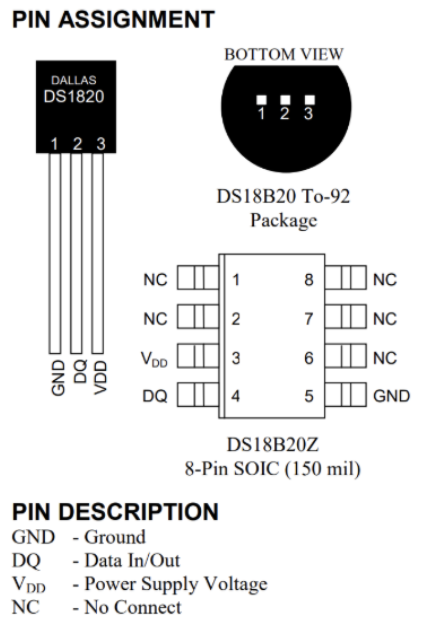
\includegraphics[width=0.7\textwidth]{temperatura.png}
		\caption{Datasheet del Sensor de Temperatura Digital DS18B20}
		\label{fig:ds18b20_datasheet}
	\end{figure}
	
	\subsubsection{Adaptador para Sensor DS18B20}
	\begin{figure}[H]
		\centering
		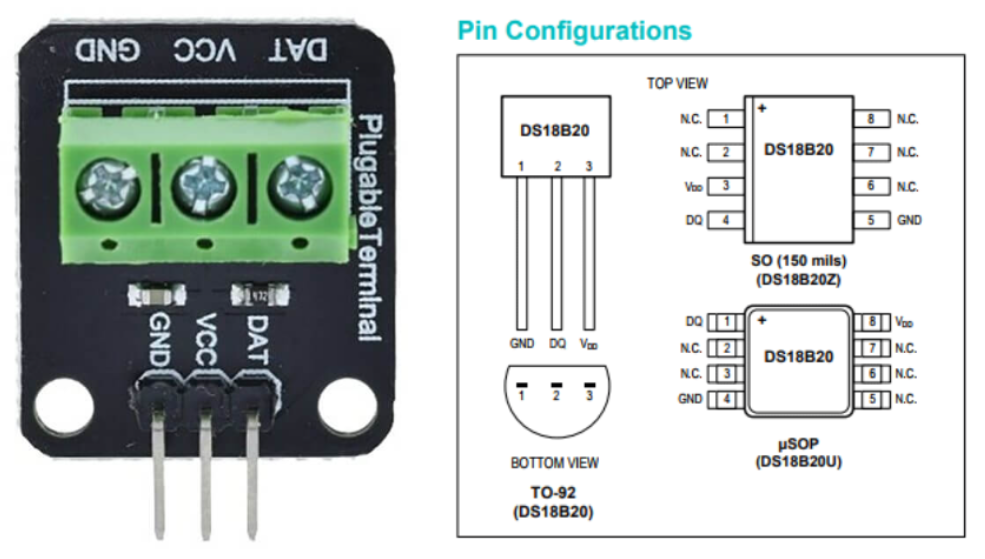
\includegraphics[width=0.8\textwidth]{adaptador.png}
		\caption{Datasheet del Adaptador para Sensor DS18B20}
		\label{fig:adaptador_ds18b20_datasheet}
	\end{figure}
	
	\subsubsection{Módulo de Sensor de pH (PH-4502C)}
	\begin{figure}[H]
		\centering
		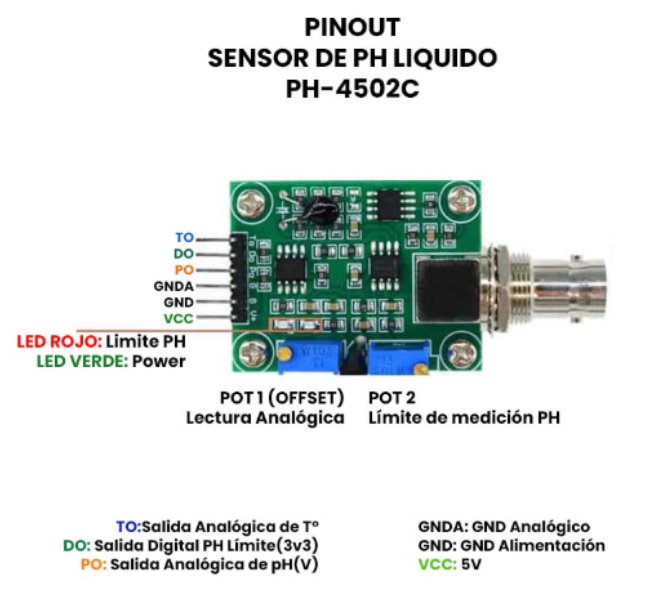
\includegraphics[width=0.8\textwidth]{ph.png}
		\caption{Datasheet del Módulo de Sensor de pH PH-4502C}
		\label{fig:ph_datasheet}
	\end{figure}
	
	\subsubsection{Electrodo E201-BNC Tipo de Sonda}
	\begin{figure}[H]
		\centering
		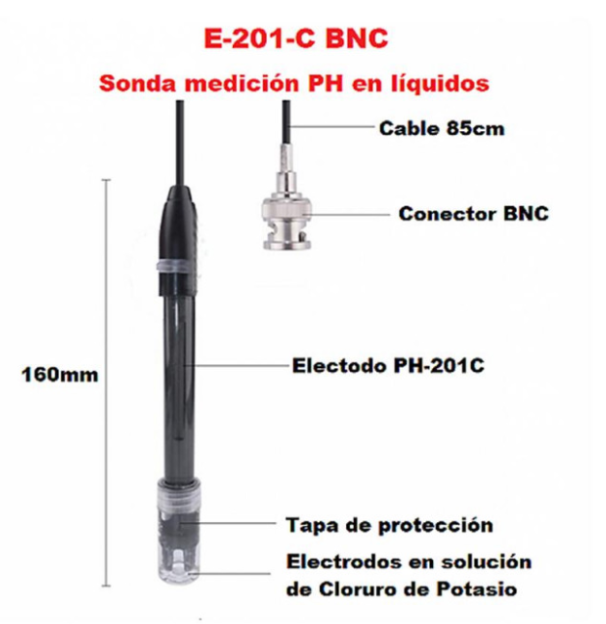
\includegraphics[width=0.8\textwidth]{electrodo.png}
		\caption{Datasheet del Electrodo de pH E201-BNC}
		\label{fig:electrodo_datasheet}
	\end{figure}
	
	\subsubsection{Display LCD TFT a Color de 1.8" (ST7735)}
	\begin{figure}[H]
		\centering
		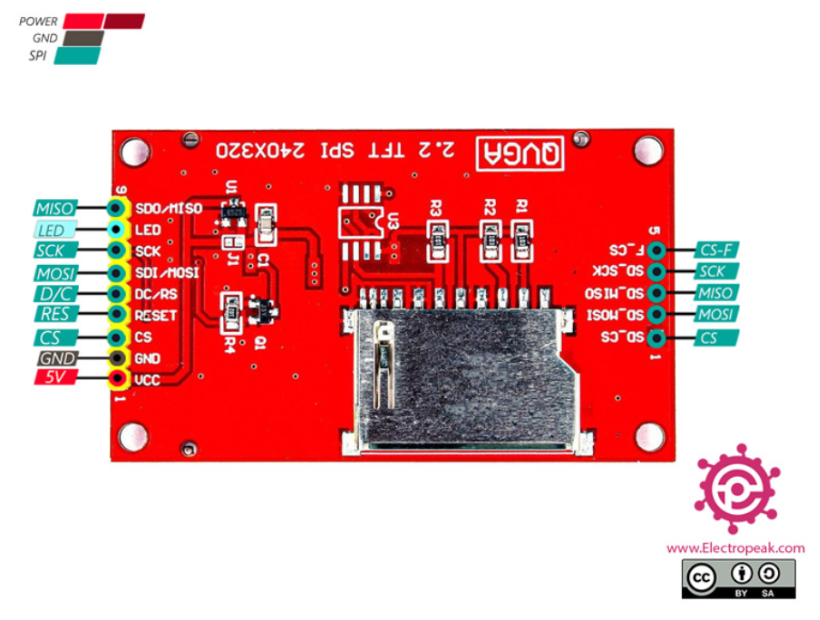
\includegraphics[width=0.8\textwidth]{display.png}
		\caption{Datasheet del Display LCD TFT ST7735}
		\label{fig:display_datasheet}
	\end{figure}
	
	\subsubsection{LED RGB}
	\begin{figure}[H]
		\centering
		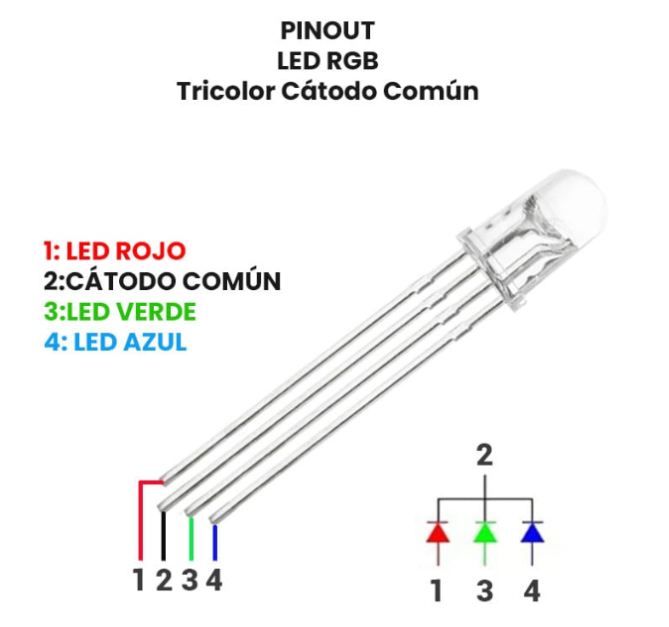
\includegraphics[width=0.8\textwidth]{rgb.png}
		\caption{Datasheet del LED RGB}
		\label{fig:rgb_datasheet}
	\end{figure}
\end{document}